% Provenance (never printed): cycle 4 SVT, "La planete Terre, l'environnement
% et l'action humaine": resources from the Earth, their geological origin, the
% time they take to form and the rate we use them; see
% sources/book1/PROVENANCE.md. Book 1, grade 9, chapter 3.
% Vocabulary guard: owns ore deposit (with concentration factor), aggregate,
% reserve. Resource, renewable resource, ore, raw material (chemistry grade
% 5), fossil fuels (chemistry grade 8) and element abundances (chemistry
% grade 9) are recalled in prose. Groundwater and aquifers are g6's. Coal,
% oil and gas are told, not defined: "source rock", "reservoir", "seal",
% "trap" and the coal ranks belong to Book 2 g11 (fossil-fuel-geology);
% "hydrothermal" is not used (later books). Scientific notation (grade 9).
\chapter{地球资源}\label{ch:g9:earth-resources}

智能手机可以放进口袋，却含有几十种化学元素：
铜用于导线，钕用于扬声器的磁铁，镓
用于屏幕的发光，铟用于屏幕上导电的薄涂层，
还有许多其他元素。它们每一种都是从地下挖出来的，
分布于地球某处。房屋用料要多得多：一户普通家庭住宅
需要约一百吨砂、\omterm{def:g3:stones-pebbles-sand:pebble}{砾石}和碎石，它
所分摊的周边街道和学校用料约为其三倍。
这些材料在地球的什么位置被发现？为什么在那里？
% ledger: usgs:smartphone, usgs:aggregate (114 and 328 short tons: about 100 and 300 t)

\begin{recall}
在化学中你已经学过：人们从自然界获取的材料是
\emph{资源}；\emph{矿石}是可从中提取金属的
\omterm{def:g3:stones-pebbles-sand:rock}{岩石}；自然界更新速度与我们使用速度相当的，是\emph{可再生}资源；
煤、油和天然气是\emph{\omterm{def:g7:sediments-and-fossils:fossil}{化石}燃料}；氧、
硅、铝和铁是\omterm{def:g6:inside-the-earth:layers}{地壳}中丰度最高的元素。
\omterm{def:g6:water-underground:groundwater}{地下水}充满\omterm{def:g6:water-underground:aquifer}{含水层}的\omterm{def:g6:water-underground:porosity}{孔隙}，雨水又使其得到补充
（\cref{ch:g6:water-underground}）。\omterm{def:g7:sediments-and-fossils:sediment}{沉积物}逐层堆积，并
变为\omterm{def:g6:rocks-and-minerals:rock-families}{沉积岩}（\cref{ch:g7:sediments-and-fossils}），所需时间
以百万年计（\cref{ch:g7:geological-time}）。
\end{recall}

\section{为什么金属必须富集}

铜无处不在：普通\omterm{def:g3:stones-pebbles-sand:rock}{岩石}中含有少量铜，
每百千克\omterm{def:g3:stones-pebbles-sand:rock}{岩石}中仅有几克。但要从这样的\omterm{def:g3:stones-pebbles-sand:rock}{岩石}中提取一千克铜，
就得开采、破碎并处理数吨\omterm{def:g3:stones-pebbles-sand:rock}{岩石}。采矿
只有在自然界已把金属富集到品位高得多的\omterm{def:g3:stones-pebbles-sand:rock}{岩石}的地方才值得。
% ledger: perkins:ore-grades (copper 0.006 % of the crust)

\begin{definition}[矿床与富集系数]\label{def:g9:earth-resources:ore-deposit}
\emph{矿床}\index{矿床}是一种岩体，其中
自然过程已将某种金属或\omterm{def:g6:rocks-and-minerals:mineral}{矿物}富集到足以
有利可图地开采的程度。\emph{富集
系数}\index{富集系数}是某金属在矿石中的含量，
为其在\omterm{def:g6:inside-the-earth:layers}{地壳}中平均含量的倍数：
\[
\text{富集系数} = \frac{\text{矿石中的含量}}{\text{地壳中的平均含量}} .
\]
\end{definition}
% ledger: perkins:ore-grades, earle:ore-grades

\omterm{def:g6:inside-the-earth:layers}{地壳}中常见的金属铝和铁，只需富集
约四倍。铜约需 80 倍，锌约需 600 倍，
而图中最稀有的金属金、锡和铬则需数
千倍。金属在\omterm{def:g6:inside-the-earth:layers}{地壳}中越稀少，自然界就越需费力地形成
其矿石，能做到这一点的地方也就越少。
% ledger: perkins:ore-grades, earle:ore-grades

\begin{example}[铜]
\omterm{def:g6:inside-the-earth:layers}{地壳}中铜的平均含量为 \qty{0.006}{\%}；铜矿石可
开采的品位约为 \qty{0.5}{\%}。\omterm{def:g9:earth-resources:ore-deposit}{富集系数}为 $0.5 \div 0.006
\approx 83$，约为 80，或接近 $10^2$。另一本教材取 \qty{40}{ppm}
（\qty{0.004}{\%}）作为普通\omterm{def:g3:stones-pebbles-sand:rock}{岩石}的含量，\qty{1}{\%} 作为矿石的含量：$1 \div
0.004 = 250$。两个数值不同，但说明的是同一件事：
铜矿石的品位约为普通\omterm{def:g3:stones-pebbles-sand:rock}{岩石}的一百倍。
\end{example}
% ledger: perkins:ore-grades, earle:ore-grades

\begin{omfigure}
\begin{tikzpicture}
\begin{axis}[xbar, xmode=log, width=12cm, height=5.3cm, xmin=1, xmax=2e4,
  log origin=infty, bar width=9pt, enlarge y limits=0.1,
  ytick=data, yticklabels={{铝},{铁},{铜},{锌},{金},{锡},{铬}},
  y dir=reverse, xlabel={富集系数（对数尺度）},
  xtick={1,10,100,1000,10000}, xticklabels={$1$,$10$,$10^2$,$10^3$,$10^4$},
  tick label style={font=\footnotesize}, label style={font=\small},
  nodes near coords, nodes near coords style={font=\scriptsize, anchor=west},
  point meta=explicit, xmajorgrids, grid style={black!12}]
\addplot[fill=omWarm!45, draw=omWarm!80!black] table[x=factor, y=x, meta=factor] {figdata/out/grade-9-concentration.dat};
\end{axis}
\end{tikzpicture}

{\small 自然界需将七种金属富集多少倍，才能形成
值得开采的矿石：矿石的最低品位除以
\omterm{def:g6:inside-the-earth:layers}{地壳}的平均含量。刻度每一步都是前一步的十倍。
数据来源：D.~Perkins 等，\emph{Mineralogy}，金的数据
来自 S.~Earle，\emph{Environmental Geology}。}
% ledger: perkins:ore-grades, earle:ore-grades (figdata/grade-9/concentration.py)
\label{fig:g9:earth-resources:factors}
\end{omfigure}

\begin{method}[计算富集系数]
\begin{enumerate}
  \item 将金属在矿石中和\omterm{def:g6:inside-the-earth:layers}{地壳}平均含量中的数值化为
        同一单位（百分数，或克每吨）。
  \item 用矿石中的含量除以\omterm{def:g6:inside-the-earth:layers}{地壳}中的含量。
  \item 对结果取整：关键在于其数量级，约为
        10、100 或 1000，可写成十的幂。
\end{enumerate}
\end{method}


\section{矿床的形成}

自然界以多种方式富集金属。其中三种如下所示。

\begin{omfigure}
\begin{tikzpicture}[x=1cm, y=1cm, font=\footnotesize, >={Stealth[length=2mm]}]
  % country rock
  \fill[black!13] (0,0) rectangle (13,4.6);
  % surface with a valley on the right
  \fill[white] (0,4.6) -- (8.4,4.6) -- (9.6,3.7) -- (11.2,3.7) -- (12.0,4.6) -- (13,4.6) -- (13,5.6) -- (0,5.6) -- cycle;
  \draw[black!60] (0,4.6) -- (8.4,4.6) -- (9.6,3.7) -- (11.2,3.7) -- (12.0,4.6) -- (13,4.6);
  % river gravels on the valley floor
  \fill[omLithCongl] (9.5,3.75) -- (11.3,3.75) -- (11.15,3.35) -- (9.65,3.35) -- cycle;
  \foreach \x in {9.8,10.1,10.45,10.8,11.05} \fill[black!45] (\x,3.6) circle (0.05);
  \foreach \x in {9.9,10.3,10.65,10.95} \fill[yellow!80!orange] (\x,3.4) circle (0.045);
  \fill[omRiver!60] (9.9,3.75) rectangle (10.9,3.85);
  % magma body (cooling granite)
  \fill[omLithGranite] (1.0,0) .. controls (1.2,1.6) and (2.2,2.1) .. (3.4,2.1)
     .. controls (4.6,2.1) and (5.6,1.6) .. (5.8,0) -- cycle;
  \draw[black!50] (1.0,0) .. controls (1.2,1.6) and (2.2,2.1) .. (3.4,2.1)
     .. controls (4.6,2.1) and (5.6,1.6) .. (5.8,0);
  % heavy minerals settled at the bottom of the magma body
  \fill[black!60] (1.05,0) rectangle (5.75,0.25);
  % cracks and veins above the magma
  \foreach \x/\a in {2.6/12, 3.4/-6, 4.3/-15} {
    \draw[black, line width=1.6pt] (\x,2.15) -- ++(90+\a:2.0);
    \draw[yellow!80!orange, line width=0.6pt] (\x,2.15) -- ++(90+\a:2.0);
  }
  % hot water rising
  \draw[->, omWarm, thick] (2.1,1.9) .. controls (1.9,2.7) and (2.2,3.2) .. (2.45,3.7);
  \draw[->, omWarm, thick] (4.95,1.7) .. controls (5.1,2.6) and (4.8,3.3) .. (4.55,3.8);
  % labels
  \node[anchor=north, align=center] at (3.4,1.35) {冷却中的岩浆体};
  \node[anchor=west, align=left, fill=white, fill opacity=0.85, text opacity=1, inner sep=1.5pt] at (6.2,0.75)
    {\textbf{1} 富含金属的重矿物 \\ 沉降至底部};
  \draw[black!70] (6.15,0.65) -- (5.5,0.15);
  \node[anchor=west, align=left, fill=white, fill opacity=0.85, text opacity=1, inner sep=1.5pt] at (5.6,2.55)
    {\textbf{2} 热水沿裂隙上升，\\ 冷却后析出金属：矿脉};
  \draw[black!70] (5.55,2.6) -- (4.2,3.3);
  \node[anchor=south, align=center] at (10.4,4.7) {\textbf{3} 金粒与河流砾石一同沉积，\\ 形成砂矿};
  \draw[black!70] (10.4,4.7) -- (10.3,3.45);
  \node[anchor=south west] at (0.1,4.65) {地表};
\end{tikzpicture}

{\small 富集金属的三种方式（示意图，非按比例）。（1）
\omterm{def:g7:volcanoes:magma}{岩浆}体中，富含镍或铜的重\omterm{def:g6:rocks-and-minerals:mineral}{矿物}下沉并聚集于
底部。（2）\omterm{def:g7:volcanoes:magma}{岩浆}加热的\omterm{def:g6:water-underground:groundwater}{地下水}，以及\omterm{def:g7:volcanoes:magma}{岩浆}自身释放的水，
溶解金属，沿裂隙上升，并在\omterm{def:g3:stones-pebbles-sand:rock}{岩石}较冷处将其沉淀，
充填裂隙形成矿脉。（3）\omterm{def:g5:water-shapes-the-land:erosion}{侵蚀}使金从
矿脉中释出；\omterm{def:g1:landscapes-around-us:water}{河流}搬运金，重的金粒\omterm{def:g5:water-shapes-the-land:deposition}{沉积}于
\omterm{def:g3:stones-pebbles-sand:pebble}{砾石}之间，直至\omterm{def:g3:stones-pebbles-sand:rock}{基岩}。}
% ledger: earle:magmatic, usgs:gold-lode, usgs:gold-placer
\label{fig:g9:earth-resources:deposits}
\end{omfigure}

\paragraph{\omterm{def:g7:volcanoes:magma}{岩浆}中。}\omterm{def:g7:volcanoes:magma}{岩浆}体冷却时，最先结晶的\omterm{def:g6:rocks-and-minerals:mineral}{矿物}
不一定是最轻的。在源自\omterm{def:g6:inside-the-earth:layers}{地幔}的\omterm{def:g7:volcanoes:magma}{岩浆}中，
富含镍和铜的重\omterm{def:g6:rocks-and-minerals:mineral}{矿物}下沉至底部，聚集成富集层。
世界上开采的镍，大多来自
此类\omterm{def:g9:earth-resources:ore-deposit}{矿床}。
% ledger: earle:magmatic

\paragraph{热水在裂隙中成矿。}\omterm{def:g7:volcanoes:magma}{岩浆}体附近流动的\omterm{def:g6:water-underground:groundwater}{地下水}，
位于地表以下数千米处，受热后沿\omterm{def:g3:stones-pebbles-sand:rock}{岩石}的
裂隙上升。热水溶解其所流经\omterm{def:g3:stones-pebbles-sand:rock}{岩石}中的金属。
当热水到达靠近地表、较冷的\omterm{def:g3:stones-pebbles-sand:rock}{岩石}时，金属
以\omterm{def:g6:rocks-and-minerals:mineral}{矿物}形式从水中析出，充填裂隙，称为
\emph{矿脉}\index{矿脉}。许多金\omterm{def:g9:earth-resources:ore-deposit}{矿床}即属此类矿脉。在
某些\omterm{def:g7:volcanoes:magma}{岩浆}体周围，热水穿过整片破碎岩体，
并在其中留下铜，分布分散，却遍布巨大体积：这些是世界上
最大的铜\omterm{def:g9:earth-resources:ore-deposit}{矿床}。
% ledger: usgs:gold-lode, earle:porphyry

\begin{omfigure}
\begin{minipage}[c]{0.46\linewidth}\centering
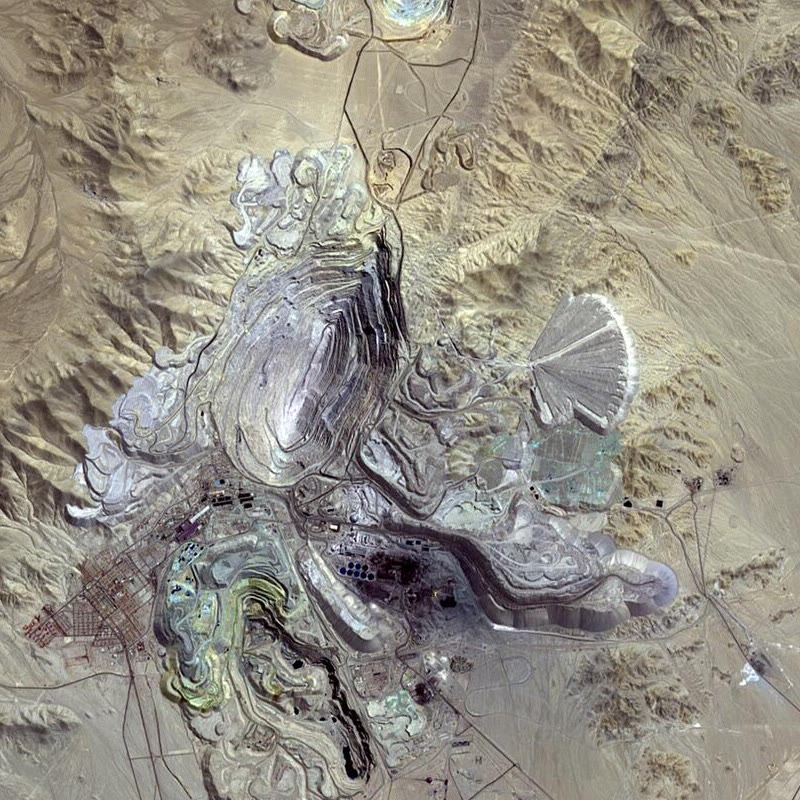
\includegraphics[width=\linewidth]{images/book1/g9-chuquicamata.jpg}
\end{minipage}\hfill
\begin{minipage}[c]{0.5\linewidth}\raggedright
{\small 智利阿塔卡马\omterm{def:g5:weather-and-climate:desert}{沙漠}中的丘基卡马塔铜矿，
于 2007 年由 NASA 卫星上的 ASTER 仪器拍摄（图像宽约
\qty{12}{km}）。中部椭圆形矿坑，开采已逾一
个世纪，长 \qty{4.3}{km}、宽 \qty{2.7}{km}、深 \qty{1.1}{km}。
NASA/METI/AIST/Japan
Space Systems and the U.S./Japan ASTER Science Team（公有领域，经由
维基共享资源）}
\end{minipage}
% ledger: commons:chuquicamata, earle:chuquicamata
\label{fig:g9:earth-resources:chuquicamata}
\end{omfigure}

\paragraph{\omterm{def:g1:landscapes-around-us:water}{河流}\omterm{def:g3:stones-pebbles-sand:pebble}{砾石}中。}金不生锈，也几乎不\omterm{def:g5:water-shapes-the-land:weathering}{风化}。当
\omterm{def:g5:water-shapes-the-land:erosion}{侵蚀}磨损金矿脉时，金以粉末、薄片、
颗粒，有时为块金的形式释出，\omterm{def:g1:landscapes-around-us:water}{河流}将其向下游搬运。金的密度很大：
纯金约为 \qty{19}{g/cm^3}，普通\omterm{def:g3:stones-pebbles-sand:rock}{岩石}约为
\qty{2.5}{g/cm^3}。\omterm{def:g5:water-shapes-the-land:flood}{洪水}期间，整个沙砾河床移动，重的
金粒下沉并聚集于\omterm{def:g3:stones-pebbles-sand:rock}{基岩}上。地质学家
称此类\omterm{def:g9:earth-resources:ore-deposit}{矿床}为\emph{砂矿}\index{砂矿}。
% ledger: usgs:gold-placer

\section{煤、石油和天然气}

煤、石油和天然气是生物的遗骸，在腐烂前
即已被埋藏。动植物死亡后，其有机物几乎全部
在数周至数十年内转化为二氧化碳。只有
与空气中的氧气隔绝的部分，位于静止沼泽或
深海底部，才能被埋藏并保存数百万年。
% ledger: earle:coal, earle:oil-gas

\begin{omfigure}
\begin{minipage}[c]{0.46\linewidth}\centering
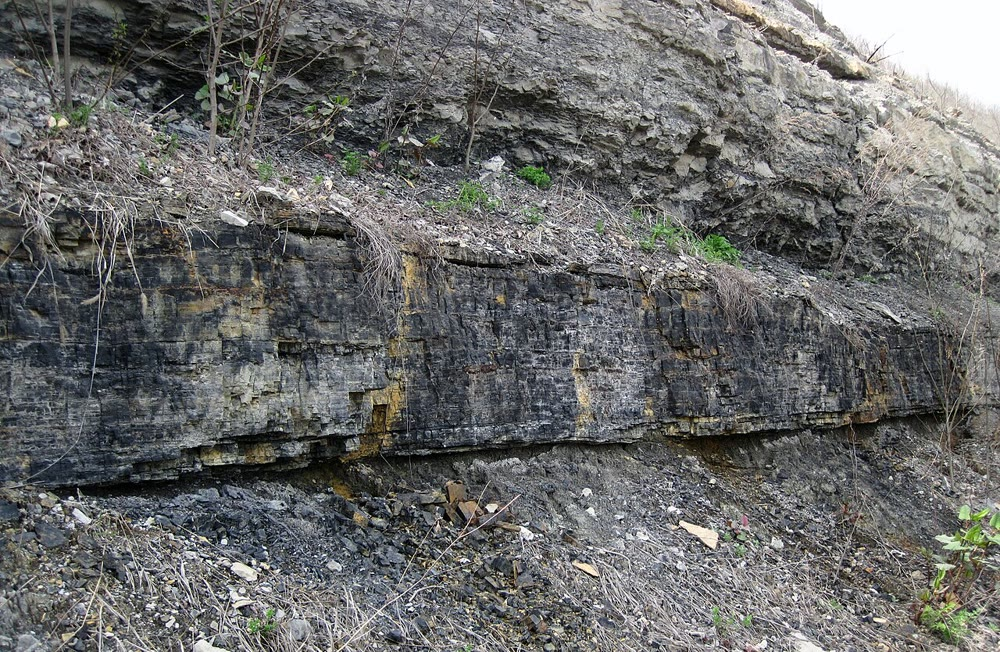
\includegraphics[width=\linewidth]{images/book1/g9-coal-seam.jpg}
\end{minipage}\hfill
\begin{minipage}[c]{0.5\linewidth}\raggedright
{\small 煤层，即中部深色的一层，夹于
\omterm{def:g6:rocks-and-minerals:rock-families}{沉积岩}之间，位于美国俄亥俄州一条道路旁。煤层
近乎水平，与当年的沼泽一致。照片：James St.~John（CC BY 2.0，经由
维基共享资源）}
\end{minipage}
% ledger: commons:meigs-coal
\label{fig:g9:earth-resources:coal-seam}
\end{omfigure}


\paragraph{煤。} 煤形成于\omterm{def:g1:landscapes-around-us:water}{河流}和\omterm{def:g5:water-shapes-the-land:delta}{三角洲}旁的沼泽中，
\omterm{def:g5:weather-and-climate:climate}{气候}温暖湿润，植物生长迅速。枯死的树干和树叶落入
含氧极少的静水中，不会腐烂。沼泽需要持续
数百年至数千年，才能堆积成厚厚的一层。某一天，一条\omterm{def:g1:landscapes-around-us:water}{河流}改道或泛滥，
将沼泽覆盖上砂和泥。随着\omterm{def:g7:sediments-and-fossils:sediment}{沉积物}不断堆积，
植物层受到挤压和加热，转变为
煤：先形成碳含量约三分之一的软褐煤，
埋深数百米；再是碳含量高达 86~\% 的硬黑煤，
埋深数千米。以今天美国开采的煤为例，
其年龄大多在 1 亿至 3 亿年之间。
% ledger: earle:coal, eia:coal

\begin{omfigure}
\begin{tikzpicture}[x=1cm, y=0.8cm, font=\footnotesize]
  \foreach \i/\t in {0/{(a) 沼泽森林：\\ 死去的植物在静水下 \\ 层层堆积},
                     1/{(b) 被河流带来的 \\ 沙和泥埋藏，\\ 这一层受到挤压},
                     2/{(c) 更深、更热 \\ （数百米）：\\ 松软的褐煤},
                     3/{(d) 再深一些 \\ （数千米）：\\ 坚硬的黑色煤}} {
    \begin{scope}[xshift=\i*3.35cm]
      \draw[black!40] (0,0) rectangle (2.9,4.2);
      \node[align=center, anchor=north, font=\scriptsize] at (1.45,-0.1) {\t};
    \end{scope}
  }
  % (a) swamp: water, trees, plant layer
  \fill[omSea] (0,2.6) rectangle (2.9,3.1);
  \fill[brown!60!black!70] (0,2.0) rectangle (2.9,2.6);
  \fill[omLithShale] (0,0) rectangle (2.9,2.0);
  \foreach \x in {0.5,1.4,2.3} {
    \draw[brown!50!black, line width=1.2pt] (\x,2.6) -- (\x,3.7);
    \fill[green!45!black] (\x,3.85) circle (0.3);
  }
  % (b) buried
  \begin{scope}[xshift=3.35cm]
    \fill[lith sandstone] (0,2.6) rectangle (2.9,4.0);
    \fill[brown!55!black!80] (0,2.2) rectangle (2.9,2.6);
    \fill[omLithShale] (0,0) rectangle (2.9,2.2);
    \draw[->, thick] (1.45,4.15) -- (1.45,3.45);
  \end{scope}
  % (c) lignite
  \begin{scope}[xshift=6.7cm]
    \fill[lith sandstone] (0,1.9) rectangle (2.9,4.2);
    \fill[brown!45!black] (0,1.65) rectangle (2.9,1.9);
    \fill[omLithShale] (0,0) rectangle (2.9,1.65);
  \end{scope}
  % (d) coal
  \begin{scope}[xshift=10.05cm]
    \fill[lith sandstone] (0,1.25) rectangle (2.9,4.2);
    \fill[black!85] (0,1.1) rectangle (2.9,1.25);
    \fill[omLithShale] (0,0) rectangle (2.9,1.1);
  \end{scope}
\end{tikzpicture}

{\small 由沼泽到煤层的演化（示意图，不按比例）。随着植物层
埋深增加，受到挤压和加热：水和气体逸出，
层厚变薄，碳的占比升高。}
% ledger: earle:coal, eia:coal
\label{fig:g9:earth-resources:coal}
\end{omfigure}


\paragraph{石油与天然气。} 石油和大多数天然气来自生活在海中的微小
动植物，如硅藻。它们的遗骸
随\omterm{def:g3:stones-pebbles-sand:sand}{泥沙}\omterm{def:g5:water-shapes-the-land:deposition}{沉积}到海底，其中一部分在腐烂前即被掩埋。
经过数百万年、\omterm{def:g7:sediments-and-fossils:sediment}{沉积物}埋深数千米后，热量和压力
使其发生变化：在约 \qty{2}{km} 以下、温度约为 60 至
\qty{120}{\degreeCelsius} 之间时转化为石油；温度更高时转化为天然气。
石油和天然气的密度比水小。它们沿透水\omterm{def:g3:stones-pebbles-sand:rock}{岩石}的\omterm{def:g6:water-underground:porosity}{孔隙}
缓慢向上运移，许多会到达地表而逸失。我们能找到的
石油和天然气则是在途中被一层不透水岩层挡住，常位于
背斜顶部并在此聚集：天然气在上，石油在其下，
再往下是水。
% ledger: eia:oil, eia:gas, earle:oil-gas

\begin{omfigure}
\begin{tikzpicture}[x=1cm, y=1cm, font=\footnotesize, >={Stealth[length=2mm]}]
  \def\fold#1{(0,#1) .. controls (3,#1+1.0) and (4.0,#1+1.6) .. (6,#1+1.6) .. controls (8.0,#1+1.6) and (9,#1+1.0) .. (12,#1)}
  % layers from the bottom up
  \fill[omLithShale!60!black!40] (0,0) -- \fold{0.9} -- (12,0) -- cycle;
  \fill[lith sandstone] \fold{0.9} -- (12,2.1) -- (12,2.1) .. controls (9,3.1) and (8.0,3.7) .. (6,3.7) .. controls (4.0,3.7) and (3,3.1) .. (0,2.1) -- cycle;
  \fill[lith shale] (0,2.1) .. controls (3,3.1) and (4.0,3.7) .. (6,3.7) .. controls (8.0,3.7) and (9,3.1) .. (12,2.1) -- (12,3.6) .. controls (9,4.6) and (8.0,5.2) .. (6,5.2) .. controls (4.0,5.2) and (3,4.6) .. (0,3.6) -- cycle;
  \fill[lith sandstone] (0,3.6) .. controls (3,4.6) and (4.0,5.2) .. (6,5.2) .. controls (8.0,5.2) and (9,4.6) .. (12,3.6) -- (12,5.6) -- (0,5.6) -- cycle;
  % gas and oil under the crest of the impermeable layer
  \fill[omWxSun!60] (4.55,3.55) .. controls (5.2,3.69) and (6.8,3.69) .. (7.45,3.55) -- (7.1,3.35) -- (4.9,3.35) -- cycle;
  \fill[black!75] (4.9,3.35) -- (7.1,3.35) -- (8.05,3.05) .. controls (7.0,3.15) and (5.0,3.15) .. (3.95,3.05) -- cycle;
  % arrows: oil creeping up through the permeable layer
  \draw[->, black, thick] (1.4,2.05) -- (2.4,2.55);
  \draw[->, black, thick] (10.6,2.05) -- (9.6,2.55);
  \draw[->, black!70] (3.0,2.65) -- (3.8,2.95);
  \draw[->, black!70] (9.0,2.65) -- (8.2,2.95);
  % labels
  \node[anchor=west, fill=white, fill opacity=0.85, text opacity=1, inner sep=1.5pt] at (0.1,0.45) {古海底的暗色泥：石油和天然气在此形成};
  \node[anchor=east, fill=white, fill opacity=0.85, text opacity=1, inner sep=1.5pt] at (11.9,1.9) {透水砂岩};
  \node[anchor=east, fill=white, fill opacity=0.85, text opacity=1, inner sep=1.5pt] at (11.9,3.25) {不透水页岩};
  \node[anchor=south, fill=white, fill opacity=0.85, text opacity=1, inner sep=1.5pt] at (6,5.25) {地表岩石};
  \node[font=\scriptsize] at (6,3.48) {天然气};
  \node[font=\scriptsize, text=white] at (6,3.22) {石油};
\end{tikzpicture}

{\small 石油和天然气截留于背斜顶部
不透水岩层之下（示意图，未按比例绘制；砂岩其余\omterm{def:g6:water-underground:porosity}{孔隙}中的水未画出）。
在褶皱下方，它们沿透水砂岩向上运移（箭头所示），
并在背斜顶部聚集：天然气在上，
石油在其下。}
% ledger: earle:oil-gas
\label{fig:g9:earth-resources:oil}
\end{omfigure}

\section{地下水}

\omterm{def:g6:water-underground:groundwater}{地下水}同样是取自地球的资源，也是我们每天都在用的资源。
与金属或煤不同，它是可以再生的：雨水补充\omterm{def:g6:water-underground:aquifer}{含水层}。
但补充很慢，只能与雨水渗入的速度相当。
若抽取速度超过补充速度，\omterm{def:g6:water-underground:aquifer}{含水层}的\omterm{def:g6:water-underground:water-table}{地下水位}就会下降，\omterm{def:g6:water-underground:spring}{水井}随之干涸
（见\cref{ch:g6:water-underground}）。\omterm{def:g6:water-underground:groundwater}{地下水}
只有在抽取速度不超过其再生速度时，才是可再生资源。
% ledger: wss:aquifer

\section{砂和砾石}

人们从地下挖出数量最多的固体材料，
既不是煤，也不是金属矿石，而是砂和\omterm{def:g3:stones-pebbles-sand:pebble}{砾石}。
% ledger: tos:sand

\begin{definition}[骨料]\label{def:g9:earth-resources:aggregate}
\emph{骨料}\index{骨料}是指建筑中使用的砂、\omterm{def:g3:stones-pebbles-sand:pebble}{砾石}和碎石，
用于混凝土、道路和铁路路基，
以及填充地基。
\end{definition}
% ledger: usgs:aggregate, tos:sand

砂大多用于制作混凝土，混凝土是砂、\omterm{def:g3:stones-pebbles-sand:pebble}{砾石}、水和水泥的混合物。
2019 年，全世界每年需要约 500 亿吨砂和\omterm{def:g3:stones-pebbles-sand:pebble}{砾石}，
即 $5 \times 10^{10}$ 吨，折合全球每人每天约 \qty{18}{kg}。
砂和\omterm{def:g3:stones-pebbles-sand:pebble}{砾石}取自陆地上的采坑、河床，
并且越来越多地取自海底。
若从\omterm{def:g1:landscapes-around-us:water}{河流}中大量采砂，流向\omterm{def:g1:landscapes-around-us:water}{海岸}的砂就会减少，下游的海滩随之受到\omterm{def:g5:water-shapes-the-land:erosion}{侵蚀}。
% ledger: tos:sand

\begin{omfigure}
\begin{minipage}[c]{0.46\linewidth}\centering
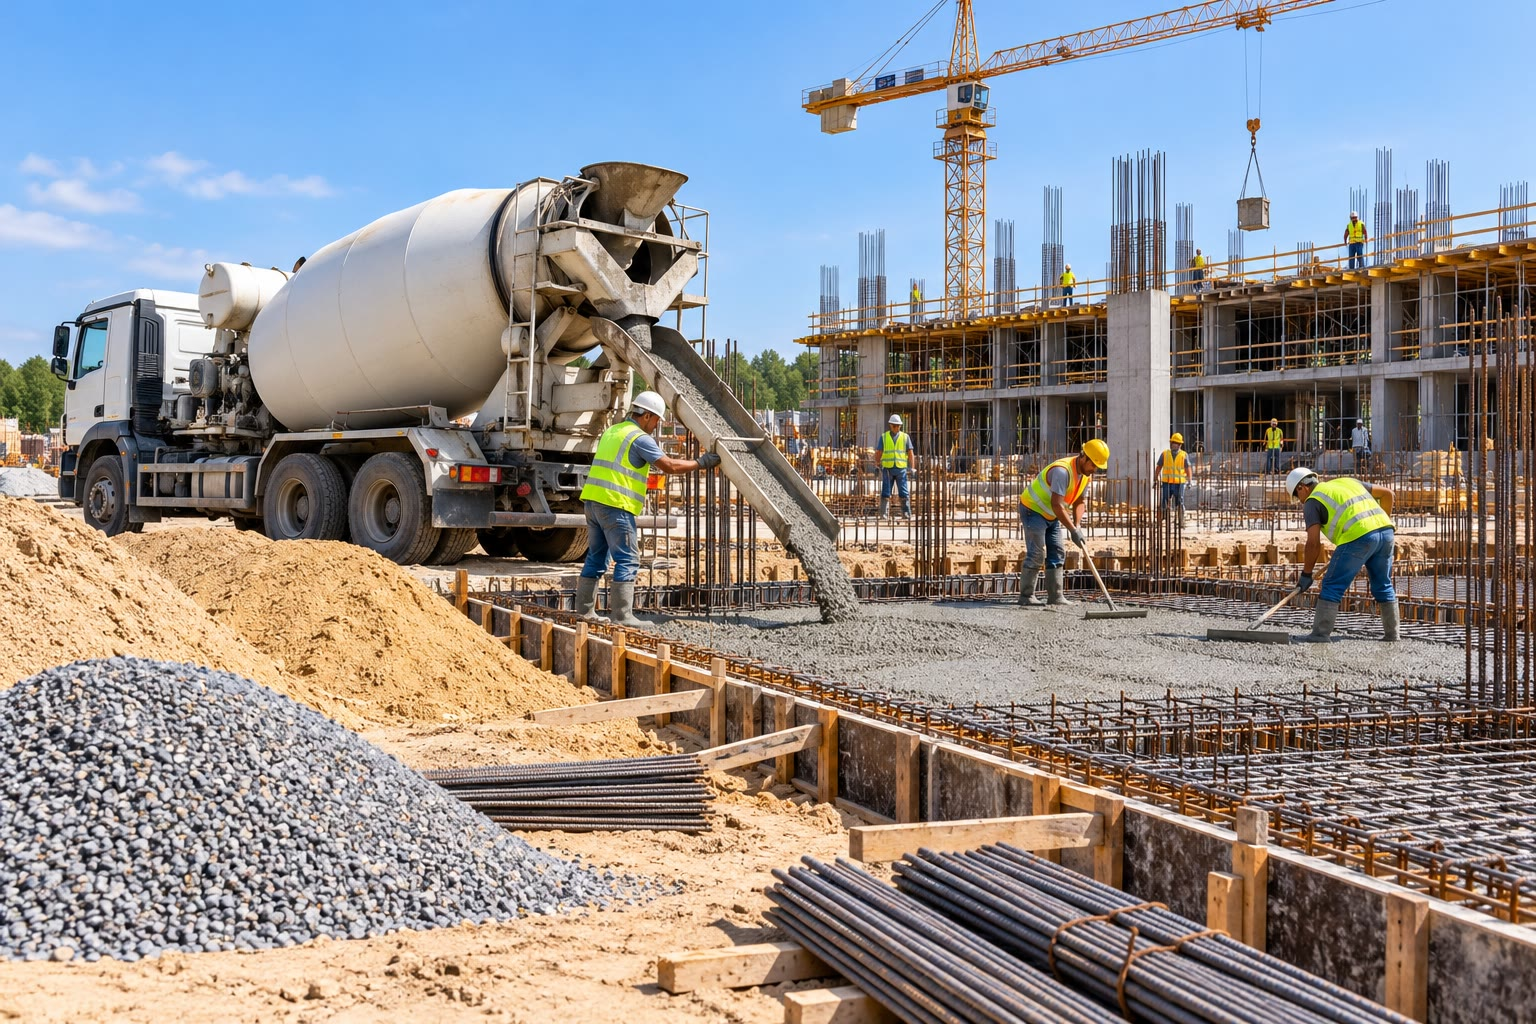
\includegraphics[width=\linewidth]{images/book1/ai/g9-building-site.jpg}
\end{minipage}\hfill
\begin{minipage}[c]{0.5\linewidth}\raggedright
{\small \omterm{def:g9:earth-resources:aggregate}{骨料}的用途：工地上堆放的砂和\omterm{def:g3:stones-pebbles-sand:pebble}{砾石}，旁边是
正在浇筑新建筑楼板的混凝土搅拌车
（AI 生成的通用场景插图）。}
\end{minipage}
\label{fig:g9:earth-resources:building-site}
\end{omfigure}

\section{可再生还是有限？}

像\omterm{def:g6:water-underground:aquifer}{含水层}中未被过度抽取的水那样，能由自然界在人类一生的时间内再生的资源，
可以永续使用。\omterm{def:g9:earth-resources:ore-deposit}{矿床}、煤层或油田的形成需要数百万年。
我们在几十年内就将其用尽，
以我们的时间尺度来看，它们根本得不到再生。
% ledger: eia:coal, earle:coal

\begin{omfigure}
\begin{tikzpicture}
\begin{axis}[xmode=log, width=12.5cm, height=4.6cm, xmin=10, xmax=1e9, ymin=0.4, ymax=4.6,
  ytick=\empty, xlabel={年（对数刻度）}, label style={font=\small},
  xtick={10,100,1000,1e4,1e5,1e6,1e7,1e8,1e9},
  xticklabels={$10$,$10^2$,$10^3$,$10^4$,$10^5$,$10^6$,$10^7$,$10^8$,$10^9$},
  tick label style={font=\footnotesize}, xmajorgrids, grid style={black!12}, clip=false]
\addplot[only marks, mark=|, mark size=4pt, line width=4pt, omWarm,
  error bars/.cd, x dir=plus, x explicit, error bar style={line width=4pt, omWarm}, error mark=none]
  table[x=lo_yr, y=y, x error expr=\thisrow{hi_yr}-\thisrow{lo_yr}] {figdata/out/grade-9-concentration-times.dat};
\node[anchor=west, font=\footnotesize, fill=white, inner sep=1pt] at (axis cs:1500,4) {沼泽形成厚层植物堆积};
\node[anchor=east, font=\footnotesize, fill=white, inner sep=1pt] at (axis cs:6e7,3) {美国开采煤炭的形成年代};
\node[anchor=west, font=\footnotesize, fill=white, inner sep=1pt] at (axis cs:150,2) {丘基卡马塔矿迄今已开采（超过一个世纪）};
\node[anchor=west, font=\footnotesize, fill=white, inner sep=1pt] at (axis cs:65,1) {按 2024 年开采速率计算的全球铜储量};
\end{axis}
\end{tikzpicture}

{\small 形成与使用的时间，刻度每一步均为前一步的十倍。
煤的形成时间约为
矿山清空一处\omterm{def:g9:earth-resources:ore-deposit}{矿床}所需时间的一百万倍。}
% ledger: earle:coal, eia:coal, earle:chuquicamata, usgs:mcs-copper (figdata/grade-9/concentration.py, part times)
\label{fig:g9:earth-resources:times}
\end{omfigure}

一种资源能维持多久？地质学家只统计已知的
且可以开采的那部分。

\begin{definition}[储量]\label{def:g9:earth-resources:reserve}
矿产资源的\emph{储量}\index{储量}是指已知\omterm{def:g9:earth-resources:ore-deposit}{矿床}中，
能够有利可图地开采的部分，
即在当时的技术与价格条件下可以开采的那部分。
\end{definition}
% ledger: usgs:mcs-reserves

\omterm{def:g9:earth-resources:reserve}{储量}并不等于地下的全部矿产。发现新\omterm{def:g9:earth-resources:ore-deposit}{矿床}、
技术改进或价格上涨时，\omterm{def:g9:earth-resources:reserve}{储量}随之增加，
\omterm{def:g9:earth-resources:ore-deposit}{矿床}被开采时，\omterm{def:g9:earth-resources:reserve}{储量}则会减少。1970 年，全球铜\omterm{def:g9:earth-resources:reserve}{储量}
估计为 2.8 亿吨。此后，约 7 亿吨铜已被开采，
相当于该\omterm{def:g9:earth-resources:reserve}{储量}的两倍半，而 2024 年的\omterm{def:g9:earth-resources:reserve}{储量}估计仍有
9.8 亿吨。
% ledger: usgs:mcs-reserves

\begin{dated}{2025}
2024 年，全球矿山共产出约 2300 万吨铜。
按此速率，9.8 亿吨的\omterm{def:g9:earth-resources:reserve}{储量}可维持 $980 \div 23
\approx 43$ 年。这个数字并非铜何时耗尽的日期，
它衡量的是今天已知且值得开采的铜。
\end{dated}
% ledger: usgs:mcs-copper (figdata/grade-9/concentration.py: 42.6 years)

与煤或石油不同，金属使用后并不会被消耗掉：
材料回收利用（化学课本中已介绍）可使其重新获得。
旧电缆、报废发动机或工厂边角料中的铜，
可以再次熔化、精炼。2024 年美国的情况是，
由废料回收得到的铜约占
所用铜总量的 \qty{35}{\%}。
% ledger: usgs:mcs-copper-scrap

\begin{omfigure}
\begin{tikzpicture}[font=\footnotesize, node distance=1.2cm,
  box/.style={draw=black!60, fill=black!4, rounded corners=2pt, align=center, minimum height=0.9cm, inner sep=3pt},
  flow/.style={-{Stealth[length=2.2mm]}, line width=0.9pt, black!70}]
  \node[box, fill=omWarm!12] (ore) at (0,0) {矿床 \\（含铜 \qty{0.5}{\%}\\的岩石）};
  \node[box] (metal) at (4.2,0) {铜金属};
  \node[box] (things) at (8.2,0) {电缆、管道、\\发动机};
  \node[box, fill=blue!8] (scrap) at (6.2,-2.1) {废料};
  \node[box, fill=black!12] (waste) at (0,-2.1) {破碎岩石 \\残余};
  \draw[flow] (ore) -- node[above] {开采、破碎} node[below] {富集} (metal);
  \draw[flow] (metal) -- node[above] {制造} (things);
  \draw[flow] (things) |- node[pos=0.25, right] {丢弃} (scrap);
  \draw[flow] (scrap) -| node[pos=0.75, left] {熔化、精炼} (metal);
  \draw[flow] (ore) -- (waste);
\end{tikzpicture}

{\small 铜金属的两条路线：一条从矿石出发，需挖掘、破碎大量\omterm{def:g3:stones-pebbles-sand:rock}{岩石}；
另一条从废料出发，熔化后重新精炼。}
\end{omfigure}

\begin{example}[回收利用所节省的岩石]\label{ex:g9:earth-resources:recycling}
含铜 \qty{0.5}{\%} 的矿石，每
吨\omterm{def:g3:stones-pebbles-sand:rock}{岩石}中含铜 \qty{5}{kg}。制得一吨铜，约需
$1000 \div 5 = 200$ 吨矿石被开采、破碎并处理，其中几乎全部
变为废石。用废料制得的每吨铜，
可使这 200 吨\omterm{def:g3:stones-pebbles-sand:rock}{岩石}留在地下——\omterm{def:g9:earth-resources:ore-deposit}{矿床}也因此维持得更久。
% ledger: perkins:ore-grades (computed)
\end{example}


\section{练习}

\begin{exercise}[$\star$]\label{exo:g9:earth-resources:1}
用括号中的正确词语填空（\omterm{def:g9:earth-resources:ore-deposit}{矿床}、\omterm{def:g9:earth-resources:ore-deposit}{富集系数}、\omterm{def:g9:earth-resources:aggregate}{骨料}、
\omterm{def:g9:earth-resources:reserve}{储量}）。（a）混凝土中所用的砂是一种 \ldots\ （b）已探明的铜中，
今天能有利可图地开采的部分，是铜的 \ldots\ （c）某\omterm{def:g3:stones-pebbles-sand:rock}{岩石}中金属
富集到足以开采，该\omterm{def:g3:stones-pebbles-sand:rock}{岩石}即为一种 \ldots\ （d）一种金属被富集的
次数，就是它的 \ldots\ 。
\end{exercise}

\begin{exercise}[$\star$]\label{exo:g9:earth-resources:2}
% ledger: earle:magmatic, usgs:gold-lode, usgs:gold-placer
下列每句描述的是哪种金属富集方式：在\omterm{def:g7:volcanoes:magma}{岩浆}中、
在热水形成的裂隙中，还是在\omterm{def:g1:landscapes-around-us:water}{河流}\omterm{def:g3:stones-pebbles-sand:pebble}{砾石}中？（a）金块位于
溪流\omterm{def:g3:stones-pebbles-sand:pebble}{砾石}之下的\omterm{def:g3:stones-pebbles-sand:rock}{基岩}上。（b）热水充填裂隙，形成
石英与金的脉体。（c）一层重的镍\omterm{def:g6:rocks-and-minerals:mineral}{矿物}位于
古老\omterm{def:g7:volcanoes:magma}{岩浆}体的底部。（d）金经\omterm{def:g5:water-shapes-the-land:erosion}{侵蚀}从矿脉中释放出来。
\end{exercise}

\begin{exercise}[$\star$]\label{exo:g9:earth-resources:3}
% ledger: earle:coal, eia:coal
将下列步骤按顺序排列：（a）植物层被河砂掩埋；
（b）树木在沼泽中生长；（c）坚硬的黑煤在地下数千米处形成；
（d）死亡的植物在静水下堆积；（e）松软的褐煤形成。
\end{exercise}

\begin{exercise}[$\star$]\label{exo:g9:earth-resources:4}
以人的一生为尺度，判断每种资源是否可再生，
用一句话说明。（a）煤。（b）\omterm{def:g6:water-underground:aquifer}{含水层}的水抽取量少于
降雨的补给量。（c）铜矿石。（d）同一\omterm{def:g6:water-underground:aquifer}{含水层}的抽取速度
是补给速度的两倍。
\end{exercise}

\begin{exercise}[$\star\star$]\label{exo:g9:earth-resources:5}
% ledger: perkins:ore-grades
计算\omterm{def:g9:earth-resources:ore-deposit}{富集系数}，再将其近似写成 10 的幂的形式：
（a）锌，\omterm{def:g6:inside-the-earth:layers}{地壳}中含量 \qty{0.007}{\%}，矿石含量 \qty{4}{\%}；（b）锡，
\omterm{def:g6:inside-the-earth:layers}{地壳}中含量 \qty{0.0002}{\%}，矿石含量 \qty{0.5}{\%}；（c）铁，
\omterm{def:g6:inside-the-earth:layers}{地壳}中含量 \qty{5.6}{\%}，矿石含量 \qty{20}{\%}。（d）为何铁
所需的富集程度如此之小？
\end{exercise}

\begin{exercise}[$\star\star$]\label{exo:g9:earth-resources:6}
% ledger: usgs:gold-placer
纯金的密度约为 \qty{19.3}{g/cm^3}，普通\omterm{def:g3:stones-pebbles-sand:rock}{岩石}约为
\qty{2.5}{g/cm^3}。（a）金比\omterm{def:g3:stones-pebbles-sand:rock}{岩石}的密度大多少倍？（b）一粒体积为
\qty{0.01}{cm^3} 的金粒和同样大小的\omterm{def:g3:stones-pebbles-sand:rock}{岩石}颗粒，质量各是多少？
（c）说明为何在\omterm{def:g5:water-shapes-the-land:flood}{洪水}中，金最终\omterm{def:g5:water-shapes-the-land:deposition}{沉积}于
\omterm{def:g3:stones-pebbles-sand:pebble}{砾石}层的底部，即\omterm{def:g3:stones-pebbles-sand:rock}{基岩}之上。
\end{exercise}

\begin{exercise}[$\star\star$]\label{exo:g9:earth-resources:7}
% ledger: perkins:ore-grades, earle:ore-grades (figdata/grade-9/concentration.py)
利用\omterm{def:g9:earth-resources:ore-deposit}{富集系数}图表回答。（a）哪些金属所需的\omterm{def:g9:earth-resources:ore-deposit}{富集系数}
超过 $10^3$？（b）铜位于哪两个 10 的幂之间？（c）
铬需要富集的程度比铝高多少倍？
（d）在七种金属中，你预计哪一种开采地点
最少？请说明理由。
\end{exercise}

\begin{exercise}[$\star\star$]\label{exo:g9:earth-resources:8}
% ledger: tos:sand
全世界每人每天约需 \qty{18}{kg} 砂和\omterm{def:g3:stones-pebbles-sand:pebble}{砾石}。
（a）每人每年需要多少吨？（b）将 500
亿吨写成科学记数法。（c）一辆卡车可装 \qty{25}{t}。
一人的份额装满它需要多少天？（d）为何从河中取砂
会使下游的海滩萎缩？
\end{exercise}

\begin{exercise}[$\star\star$]\label{exo:g9:earth-resources:9}
% ledger: earle:oil-gas, eia:oil
（a）石油和天然气大多来自哪类生物？（b）在约
\qty{2}{km} 深度以下，石油在什么温度范围内形成？（c）为何石油和天然气
会在岩层中向上运移？（d）什么样的\omterm{def:g3:stones-pebbles-sand:rock}{岩石}能阻挡它们，并
使它们在何处聚集？
\end{exercise}

\begin{exercise}[$\star\star$]\label{exo:g9:earth-resources:10}
% ledger: earle:chuquicamata
丘基卡马塔矿在超过 100 年的时间里，共产出
2900 万吨铜。（a）将 2900 万吨写成科学记数法。（b）
大致估算每年的平均产量是多少？（c）若矿石含铜 \qty{1}{\%}，
为得到 2900 万吨铜，需挖出多少吨矿石？请用科学记数法表示。（d）
为何这样一座贫矿矿山
必须规模如此之大？
\end{exercise}

\begin{exercise}[$\star\star\star$]\label{exo:g9:earth-resources:11}
% ledger: usgs:mcs-reserves, usgs:mcs-copper
1970 年，全球铜\omterm{def:g9:earth-resources:reserve}{储量}估计为 2.8 亿吨。
1970 年至 2024 年间，约开采了 6.97 亿吨，而
2024 年的\omterm{def:g9:earth-resources:reserve}{储量}为 9.8 亿吨，2024 年开采了 2300 万吨。
（a）若 1970 年的\omterm{def:g9:earth-resources:reserve}{储量}就是全部的铜，它将于何时
耗尽？请与已开采量作比较。（b）2024 年的\omterm{def:g9:earth-resources:reserve}{储量}是
1970 年的多少倍？（c）按 2024 年的开采速率计算，
2024 年的\omterm{def:g9:earth-resources:reserve}{储量}可维持多少年？（d）给出两条理由，说明
\omterm{def:g9:earth-resources:reserve}{储量}在开采时仍可能增长。
\end{exercise}

\begin{exercise}[$\star\star\star$]\label{exo:g9:earth-resources:12}
% ledger: earle:coal, eia:coal
一个煤层的年龄为 $3 \times 10^8$ 年。其沼泽持续了 $2 \times 10^3$
年，该煤层将在 50 年内采尽。（a）将 50 年写成
科学记数法。（b）沼泽存续的时间是开采时间的
多少倍？（c）煤层的年龄是开采时间的多少倍？
（d）利用这些数据，解释煤为何被称为
不可再生资源。
\end{exercise}

\section{问题：新城镇的混凝土}

\begin{problem}[{周末问题——一座新城镇用当地一个砂坑的
砂建成；最终答案为该砂坑砂储量
可维持的年数}]
\label{pb:g9:earth-resources:1}
% ledger: usgs:aggregate (about 100 and 300 t per home), tos:sand (figdata/grade-9/concentration.py, part problem: exercise data)
拟于十年内在一处旧砂坑附近建成一座含 \num{2000} 户住宅的新城镇，
该砂坑开挖于\omterm{def:g1:landscapes-around-us:water}{河流}阶地的\omterm{def:g3:stones-pebbles-sand:pebble}{砾石}层中。计入其分摊的
街道、学校和商店用地后，每户住宅约需 \qty{300}{t} \omterm{def:g9:earth-resources:aggregate}{骨料}，其中
\qty{40}{\%} 为砂。该砂坑的砂层
长 \qty{1.2}{km}、宽 \qty{500}{m}、厚 \qty{5}{m}；每立方米
砂的质量为 \qty{1.6}{t}。该砂坑还每年向区域其余地区
出售 \num{136000} 吨砂。

\noindent\textbf{第一部分——需要多少砂？}\par\nopagebreak
\begin{enumerate}[beginpenalty=10000]
  \item 单栋家庭住宅约需 \qty{100}{t} \omterm{def:g9:earth-resources:aggregate}{骨料}。将
        该质量以千克为单位写成科学记数法。
  \item 整座城镇共需多少吨\omterm{def:g9:earth-resources:aggregate}{骨料}？
  \item 这些\omterm{def:g9:earth-resources:aggregate}{骨料}按十年计，每年需多少吨？
  \item 该城镇每年需多少吨砂？
\end{enumerate}

\noindent\textbf{第二部分——砂\omterm{def:g9:earth-resources:reserve}{储量}。}\par\nopagebreak
\begin{enumerate}[resume, beginpenalty=10000]
  \item 计算砂层的体积，以立方米为单位，
        并写成科学记数法。
  \item 砂层的三分之一位于一处村庄和一条道路之下，
        不予开采。可开采的体积是多少？
  \item 该\omterm{def:g9:earth-resources:reserve}{储量}的质量为多少吨？
  \item 该砂坑每年向城镇与区域
        合计出售多少吨砂？
\end{enumerate}

\noindent\textbf{第三部分——是否可再生？}\par\nopagebreak
\begin{enumerate}[resume, beginpenalty=10000]
  \item 每年\omterm{def:g1:landscapes-around-us:water}{河流}向该地区带来约 \num{2000} 吨新砂，
        该砂坑的出售量是新砂量的多少倍？
  \item 以城镇的使用时间尺度而言，这种砂是否为可再生
        资源？请说明理由。
  \item 若城镇用破碎的旧混凝土替代四分之一的砂，
        每年可节省多少吨砂？
  \item 若不进行这种回收利用，该砂坑的砂\omterm{def:g9:earth-resources:reserve}{储量}
        可维持多少年？
\end{enumerate}
\end{problem}
